\documentclass{article}
\title{Applications of Graph Theory and Combinatorics in Computer Science}
\author{Dylan Galea}

\usepackage{cite}
\usepackage{amsmath}
\usepackage{amsthm}
\usepackage{amssymb}
\usepackage{physics}
\usepackage{tikz}
\usetikzlibrary{arrows.meta,automata,positioning}

\newtheorem{theorem}{Theorem}[subsection]
\newtheorem{definition}{Definition}[subsection]
\newtheorem{lemma}[definition]{Lemma}
\newtheorem*{remark}{Remark}

\begin{document}
\maketitle
\newpage
\tableofcontents
\newpage
\section{Introduction}
\newpage
\section{The Travelling Salesman Problem}
\subsection{Basic Definitions and Results}
To define the Travelling Salesman Problem, first the concept of a Hamiltonian Cycle must be defined. This concept is defined in definition \ref{Hamiltonian Cycle} below.
\begin{definition}[Hamiltonian Cycle]
\label{Hamiltonian Cycle}
Given a graph G(V,E), a Hamiltonian Cycle C in G is a cycle in G such that $\forall$ v $\in$ V(G) then v $\in$ V(C) and v appears only once in C (except the first vertex because it needs to be visited again to complete the cycle). A graph that contains a Hamiltonian cycle is called a Hamiltonian Graph. \cite{weisstein_2018}
\end{definition}
The Travelling Salesman problem can now be defined as shown in definition \ref{Travelling Salesman Problem} below.
\begin{definition}[Travelling Salesman Problem]
\label{Travelling Salesman Problem}
Suppose a simple positively weighted graph G(V,E) is given with the property that $\forall$ v,w $\in$ V ,v $\ne$ w $\implies$ $\{v,w\}$ $\in$ E, then the Travelling Salesman Problem is the task of finding a minimum weight Hamiltonian Cycle in G \cite{geeksforgeeks_2018}.
\end{definition}
To understand the Travelling Salesman Problem defined in definition \ref{Travelling Salesman Problem} , the following example is constructed :\\
\textbf{Example} : Consider the graph G below :


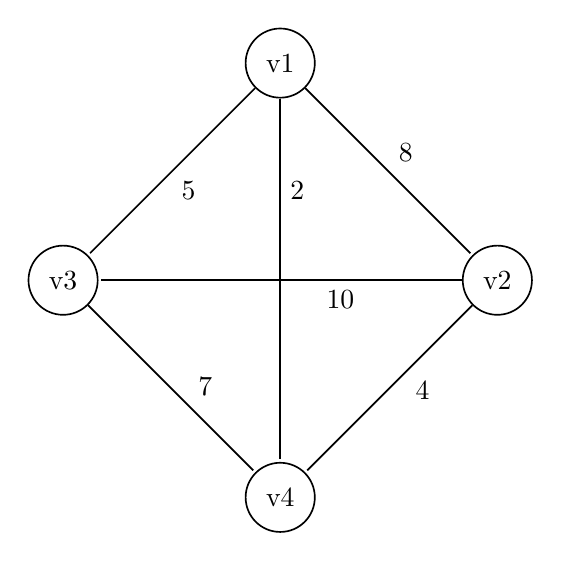
\begin{tikzpicture}[
    > = , % arrow head style
    shorten > = 1pt, % don't touch arrow head to node
    auto,
    node distance = 3cm, % distance between nodes
    semithick % line style
    ]

    \tikzset{every state}=[
    draw = black,
    thick,
    fill = white,
    minimum size = 1mm
    ]

    \node[state] (v1) {v1};
    \node[state] (v2) [below right=of v1] {v2};
    \node[state] (v3) [below left=of v1] {v3};
    \node[state] (v4) [below right=of v3] {v4};
  
    \path[->] (v1) edge  node[] {8} (v2);
    \path[->] (v1) edge  node[pos=0.5,below right] {5} (v3);
    \path[->] (v1) edge  node[pos=0.2,below right] {2} (v4);
    \path[->] (v2) edge  node[pos=0.4,below right] {10} (v3);
    \path[->] (v2) edge  node[pos=0.4,below right] {4} (v4);
    \path[->] (v3) edge  node[pos=0.6,above right] {7} (v4);
    \end{tikzpicture}

Then using definition \ref{Hamiltonian Cycle} the distinct Hamiltonian Cycles(Hamiltonian Cycles not using the exact same edges) in G are  :\\
1. (v1 v3 v4 v2 v1) with cost 24\\
2. (v1 v3 v2 v4 v1) with cost 21\\
3. (v1 v2 v3 v4 v1) with cost 27\\
Thus using definition \ref{Travelling Salesman Problem}, the answer for the Travelling Salesman Problem on this graph instance would be (v1 v3 v2 v4 v1), because it is the minimum weight Hamiltonian Cycle in G. Note that the number of distinct Hamiltonian cycles in $K_4$ is 3, and this fact is proved in general for any $K_n$ in lemma \ref{running_time}
\newpage
After illustrating the Travelling Salesman Problem using an example, some basic results are needed to be proved so that no assumptions are taken. In fact, definition \ref{Travelling Salesman Problem} suggests that in the Travelling Salesman Problem it is already known that the graph to be evaluated is Hamiltonian, this must be true because otherwise a minimum weight Hamiltonian Cycle can never be found.This uncertainty can be removed by proving that any complete graph on more than 3 vertices is Hamiltonian because the TSP is defined on complete graphs. This fact is proved in lemma \ref{Kn is Hamiltonian} below.
\begin{lemma}
\label{Kn is Hamiltonian}
For n $\geq$ 3, The complete graph on n vertices is Hamiltonian
\end{lemma}
\begin{proof}
Let $K_n$ be the complete graph on n $\geq$ 3 vertices labelled v1,v2,...,vn. Order all the vertices in the order v1,v2,...,vn with no repetitions of vertices.Then C=(v1 v2 ... vn v1) must be a cycle in $K_n$ because $\forall$ vi,vj $\in$ C, vi $\ne$ vj $\implies$ $\{vi,vj\}$ $\in$ E($K_n$). Also since $\forall$ v $\in$ V($K_n$) $\implies$ v $\in$ V(C) with only one occurence in C(except for v1 which has 2 occurences) then C must be a Hamiltonian Cycle in $K_n$ . Thus $K_n$ must be Hamiltonian.
\end{proof}
Since every $K_n$ for n $\geq$ 3 vertices is Hamiltonian this suggests that in order to find the minimum weight Hamiltonian cycle one could compute every Hamiltonian cycle in $K_n$ and then return the cycle of least cost. However, this is infeasible because this algorithm generates $\frac{(n-1)!}{2}$ distinct Hamiltonian cycles(proved in  lemma $\ref{running_time}$ below) . Thus the algorithm would have a time complexity O(n!) making it very infeasible to compute in reasonable time.\cite{geeksforgeeks_2018}
\begin{lemma}
\label{running_time}
For n $\geq$ 3 the complete graph on n vertices has $\frac{(n-1)!}{2}$ distinct Hamiltonian cycles
\end{lemma}
\begin{proof}
Let $K_n$ be the complete graph on n $\geq$ 3 vertices .Since $\forall$ u,v $\in$ V($K_n$), u $\ne$ v $\implies$ $\{u,v\}$ $\in$ E($K_n$), then every permutation of V($K_n$) must represent a Hamiltonian Cycle in $K_n$ and vice versa(1-1 correspondence). Now on n vertices there are n! possible permutations, thus due to the 1-1 correspondence we have n! Hamiltonian Cycles. However, different permutations of V($K_n$ ) may represent the same Hamiltonian Cycle in $K_n$, since the same edges would be used from E($K_n$) but in a different order of the vertices. In fact, consider the Hamiltonian Cycle C represented by the permutation (v1 v2...vn). In terms of Hamiltonian cycles, the permutation (v1 v2 ...vn) is the same as the permutation (v2...vn v1) because the same edges in E($K_n$) are used.Thus for each Hamiltonian cycle in $K_n$ we can have n permutations representing the same cycle each starting from a different vertex, but using the same edges. However,for each of these n permutation representations, the reverse of each of the permutations represent the same Hamiltonian Cycle with the difference being that the cycle is traversed in reverse order, thus we have 2n permutations representing the same Hamiltonian Cycle. Thus the number of distinct permutations is $\frac{n!}{2n}$ = $\frac{(n-1)!}{2}$. \cite{mathematics_stack_exchange_2012}
\end{proof}
Lemma \ref{running_time} confirms the difficulty in writing an algorithm that computes the minimum weight Hamiltonian cycle in brute force. The reason is because, as the number of vertices in the graph increase, the execution of the algorithm increases in a factorial manner. It is believed that the TSP does not have an algorithm that can solve the problem in polynomial time. This leads to a discussion on the different classes of problems including NP-Completness in the next sub-section with the aim to prove that TSP is NP-Complete. This would then confirm that so far no polynomial time algorithm for TSP exists.
\subsection{The classes P,NP and NP-Complete}
It is known that not all problems in the universe can be solved by algorithms even if a lot of time is dedicated to them . In fact Alan Turing proved this by proposing the Halting problem which is a problem that proveably cannot be solved by any computer. In addition to this class of problems there is the class of NP-Complete problems(NPC). For problems in this class, no polynomial time algorithm has yet been discovered , but at the same time no one was able to prove that such a polynomial time algorithm exists or not for them.What is of great interest is that if an NP-Complete problem is solved in polynomial time, then all NP-Complete problems can be solved.  In what follows, the important classes of problems will be discussed more formally, describing in the process how to prove that a problem is in NPC so that it can be proved that TSP is NP-Complete.  \cite{geeksforgeeks_2018_2}\\
\\
The three most important classes of problems are called P,NP and NP-Complete (NPC). Firstly, problems belonging to P are problems that can be solved in polynomial time and thus are tractable. Such problems can be solved by algorithms that can complete their execution in a reasonible time. Secondly, the class NP consists of decision problems that can be verified in polynomial time . This means that given a certificate(answer) to a problem in NP , this certificate can be checked in polynomial time to verify if it is correct or not. Thirdly, a decision problem is in the class NPC if it is in NP and it is as hard as any problem in NP(this will be made more clear in the next paragraph when discussing how to compare problems' complexity using reductions). Thus when proving that a problem is NP-Complete a statement is being made as to how hard is that problem and thus that no efficient algorithm exists. It must be noted that according to the definitions , in order to be in the classes NP and NPC the problems must be decision problems. Decision problems are problems for which the answer to that problem is either a yes or a no.Considering decision problems is of great benefit because decision problems are much easier to reason about and all problems in the universe can be converted to a decision problem which is as hard as the original problem and vice-versa.For example, TSP can be converted to the decision problem, "Is there a Hamiltonian cycle in $K_n$ having length k or less ?". Thus, an optimization problem can be solved in polynomial time $\iff$ it's corresponding decision problem can be solved in polynomial time.  \cite{cormen_leiserson_rivest_stein}, \cite{problems_in_computer_science} \\
\\
Thus,reasoning on whether a problem is as hard as any other problem, is as hard as conducting the same reasoning on their decision versions. Checking whether a decision problem is as hard as another decision problem can be done using reduction algorithms. Suppose that 2 decision problems A and B are given, were $\alpha$ is the input given to the algorithm solving decision problem A and $\beta$ is the input to the algorithm solving decision problem B. Then a reduction algorithm transforms any input $\alpha$ of A into some input $\beta$ of B such that the transformation takes polynomial time and the answers are the same. This means the answer for the decision problem A given $\alpha$ is 'yes' $\iff$ the answer for the decision problem B given $\beta$ is 'yes'. Thus if a decision problem A is required to be solved in polynomial time and it is known that a decision problem B can be solved in polynomial time , then A can be solved in polynomial time if a reduction algorithm can transform every input of A to an input of B since transforming this instance would take polynomial time and runnning the algorithm on this transformed instance takes also polynomial time . Thus the total number of time is polynomial . Note that this could only be done if one problem can be transformed into an other , since it is only then that 'yes' result for one is a 'yes' result for the other. Thus, the definition of NPC can now be seen more clear because it was stated that a problem A in NPC must be as hard as any problem in NP. This means that any problem in NP can be reduced using a reduction algorithm in polynomial time to A. \cite{geeksforgeeks_2018_2}, \cite{cormen_leiserson_rivest_stein}\\
\\
The previous 2 paragraphs suggest that to show that a problem A is in the class of NP-Complete problems, one must prove that first A is in NP and then that every problem in NP can be reduced using a reduction algorithm to A. Showing that A is in NP is done by checking that any given solution for A can be verified in polynomial time. Checking that every problem in NP reduces to A using a reduction algorithm is more complex because every problem in NP must be checked. However, this can be done differently by taking a known NP-Complete problem B and reduce it to A . If this reduction is done in polynomial time , then by transitivity of reductions, since every NP problem can be polynomially reduced to B , then every NP problem can be polynomially reduced to A and hence A must be NP-Complete . This argument is used in Theorem \ref{TSP is NPC} below , to show that the Travelling Salesman Problem is NP-Complete. \cite{geeksforgeeks_2018_2}

\begin{theorem}
\label{TSP is NPC}
The Travelling Salesman Problem is NP-Complete.
\end{theorem}
\begin{proof}
For the Travelling Salesman Problem to be NP-Complete it must be shown that it is in NP and that every problem in NP can be polynomially reduced to it.\\
\\
\textbf{The Travelling Salesman Problem is in NP}:\\
First , TSP must be converted to it's decision problem counterpart. The decision problem equivalent to the original TSP definition \ref{Travelling Salesman Problem} is "Does $K_n$ have a Hamiltonian Cycle of length k or less?". Thus given a particular instance to this problem(i.e. a complete graph on n-vertices to be evaluated), any answer(certificate) to the problem is some tour v1,v2,...,vn. Thus the verification mechanism must check that all the vertices of the input graph are in the certificate with no repetitions, and check that the total sum of the edges is at most k. If this is true the verification algorithm returns yes , otherwise it returns no . Checking that all the vertices are in the certificate with no repetition can be done by keeping an array of size n initialized all zeros . Thus if element i in the array is 0 it means it have not yet been encountered in the certificate and 1 otherwise . Thus, for every vertex $v_i$ in the certificate the verification algorithm checks that the array element i is set to 0 (done in O(1) time) , then if it is set to 0 the array element i is set to 1(taking O(1) time). Otherwise if element i is already set to 1 it means that the certficate has repetitions , thus the verification algorithm returns false.Therefore, this part of the verification has a time complexity O(n), which is polynomial. Then, after all vertices of the certificate have been visited the array must be traversed to check if all the elements are set to 1 .If this is not the case then the certificate contains missing vertices.The overall procedure thus has a time complexity of O(n) which is clearly polynomial . After checking that all vertices are in the certificate with no repetitions the verification algorithm must check that the tour length is less than or equal to k . This verification can be also done with a time complexity O(n) by traversing every pair of vertices. Thus the verification algorithm takes polynomial time to complete .\\
$\therefore$ The travelling Salesman Problem is in NP. \cite{cormen_leiserson_rivest_stein}, \cite{rowell}\\
\\
\textbf{Every problem in NP can be polynomially reduced to TSP}\\
To show that TSP is NP-Complete , the bold statement above is what remains to be proved. This will be carried out as described before , by taking a known NP-Complete problem and polynomially reduce it to TSP. According to Theorem 34.13 in \cite{cormen_leiserson_rivest_stein}, the Hamiltonian cycle problem is NP-Complete. Now let G(V,E) be a simple undirected graph input(instance) to the Hamiltonian Cycle problem, an instance to the TSP can be transformed from G as the following:\\
Let G'(V',E') be the complete graph obtained from G such that V'=V and E' = $\{$\{i,j\}$ : i,j \in V , i \ne j \}$. Constructing the edges in this way clearly takes polynomial time , because the complete graph on n = $\abs{V}$ has $\frac{n(n-1)}{2}$ edges. Define also the cost function :\\
c$\colon$ V'$\times$V'$\to$ $\{0,1\}$ , c(i,j) = $\begin{cases} 0& \text{if } (i,j) \in E\\ 1              & \text{otherwise} \end{cases}$\\
The above function can also be created in polynomial time , because the total number of edges that can be created is $\frac{n(n-1)}{2}$. Thus the inputs to TSP are G'(V',E'), c, k=0 ,where this whole instance can be created from G(V,E) in polynomial time. Therefore it remains to be shown that G has a Hamiltonian Cycle h $\iff$ G' has a Hamiltonian cycle of cost at most 0. Suppose that G has a Hamiltonian cycle h , then every edge of h is in E and therefore it must be a hamiltonian cycle of length 0 in G'. Conversely suppose G' has a hamiltonian cycle h' of cost at most 0 , then every every edge of h' is in E\\
$\implies$ h' is a hamiltonian cycle in G.\\
$\therefore$ the presented construction is a polynomial time reduction algorithm and thus by transitivity of reduction algorithms , every problem in NP can be reduced to TSP.\\
\\
$\therefore$ it can be concluded that TSP is NP-Complete. \cite{cormen_leiserson_rivest_stein}
\end{proof}
Theorem \ref{TSP is NPC} confirms that TSP is an NP-Complete problem . This means that no polynomial time algorithm has been discovered so far for TSP. This implies that the only option remaining is to use approximation algorithms or heuristics that are guaranteed to run in polynomial time. The next section presents some of the heustics that can be applied to the TSP , along with some theoretical results about them.
\newpage
\section{Heuristics}
\newpage
\section{Conclusion}
\newpage
\bibliography{bibliography}
\bibliographystyle{IEEEtran}
\end{document}